\section{导数}\label{zhang_derivative}
\subsection{定义}
导数的概念从物理发展出来的。
$$v\left(t_0\right)=\lim\limits_{\vartriangle t\to 0}\frac{s\left(t_0+\vartriangle t\right)-s\left(t_0\right)}{\vartriangle t}$$
\begin{figure}[htp]
  \centering
  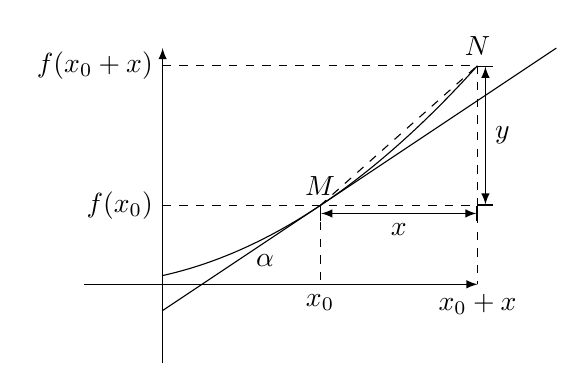
\begin{tikzpicture}[>=latex]
    \draw[->](0,0)--(5,0);
    \draw[->](1,-1)--(1,3);
    \draw[domain=1:5,samples=1000] plot(\x,{(\x^2)/9});
    \draw[domain=-2:3,samples=1000] plot(\x+3,{\x*(2/3)+1});
    \draw[dashed] (3,{(3^2)/9})--(3,0)node[below]{$x_0$};
    \draw[dashed] (3,{(3^2)/9})node[above]{$M$}--(5,{(5^2)/9})node[above]{$N$};
    \draw[dashed] (5,{(5^2)/9})--(5,0)node[below]{$x_0+\vartriangle x$};
    \node at (2.3,.5)[below]{$\measuredangle \alpha$};
    \draw[dashed] (1,{(3^2)/9})node[left]{$f(x_0)$}--(3,{(3^2)/9})--(5,{(3^2)/9});
    \draw[|<->|] (3,{(3^2)/9-.1})--(4,{(3^2)/9-.1})node[below]{$\vartriangle x$}--(5,{(3^2)/9-.1});
    \draw[dashed] (1,{(5^2)/9})node[left]{$f(x_0+\vartriangle x)$}--(5,{(5^2)/9});
    \draw[|<->|] (5.1,{(3^2)/9})--(5.1,{((5^2/9)+(3^2/9))/2})node[right]{$\vartriangle y$}--(5.1,{(5^2)/9});
\end{tikzpicture}
\end{figure}
$$NM\mbox{斜率}=\tan \beta=\frac{f\left(x_0+\vartriangle x\right)-f(x_0)}{\vartriangle x}=\frac{\vartriangle y}{\vartriangle x}$$
$$\mbox{斜率}k=\tan \alpha=\lim\limits_{\vartriangle x\to 0}\tan \beta=\lim\limits_{\vartriangle x\to 0}\frac{\vartriangle y}{\vartriangle x}=\frac{f\left(x_0+\vartriangle x\right)-f(x_0)}{\vartriangle x}$$
\subsubsection{导数定义}
$y=f(x)$在$x_0$的某邻域内有定义\\
给自变量的增量$\vartriangle x,\left(x_0+\vartriangle x\right)$仍在定义域内\\
函数得到了相应增量$\vartriangle y ,\vartriangle y =f\left(x_0+\vartriangle x\right)$\\
如果$\lim\limits_{\vartriangle x\to 0}\frac{f\left(x_0+\vartriangle x\right)-f(x_0)}{\vartriangle x}$存在,称$y=f(x)$在$x=x_0$处可导 \\
$\left(\mbox{极限值为}y=f(x)\mbox{在}x=x_0\mbox{处导数}\right)$
\begin{center}
  记$y'|_{x=x_0}=f'(x_0)=\lim\limits_{\vartriangle x\to 0}\frac{f(x_0+\vartriangle x)-f(x_0)}{\vartriangle x}$
  $$\lim\limits_{\vartriangle x\to 0}\frac{f(x_0+\vartriangle x)-f(x_0)}{\vartriangle x}\Leftrightarrow\lim\limits_{\vartriangle x\to x_0}\frac{f(x)-f(x_0)}{x-x_0}$$
\end{center}
\subsubsection{导函数定义}
$f(x)$在区间$I$内任意一点均可导。\\
$f'(x)=\lim\limits_{\vartriangle x\to 0}\frac{f(x_0+\vartriangle x)-f(x_0)}{\vartriangle x}$\\
称$f'(x)$为$y=f(x)$在区间$I$上的导函数
\subsubsection{闭区间可导定义}
$f(x)$在$[a,b]$可导$\Leftrightarrow\begin{cases}
  f'(x_0)  &x_0\in(a,b)\Leftrightarrow\begin{cases}
    \mbox{左导数}f_-'(x_0)=\lim\limits_{\vartriangle x\to 0^-}\frac{f(x_0+\vartriangle x)-f(x_0)}{\vartriangle x}\\
    \mbox{右导数}f_+'(x_0)=\lim\limits_{\vartriangle x\to 0^+}\frac{f(x_0+\vartriangle x)-f(x_0)}{\vartriangle x}
  \end{cases}\\
  f_+'(a) &x=a\\
  f_-'(a) &x=b
\end{cases}$
\subsubsection{导数与连续}
\begin{align}\label{derivative_continuity}
  f'(x)\mbox{存在}\Rightarrow f(x)\mbox{在}x=x_0\mbox{处连续}
\end{align}
\subsection{幂数,指数,对数}
\begin{align}
&\frac{d}{\mathrm{d}{x}}C = 0\label{derivative_1} \\
&\frac{d}{\mathrm{d}{x}}x^a = ax^{a-1} \label{derivative_2} \\
&\frac{d}{\mathrm{d}{x}}a^x = a^x\ln a \label{derivative_3}\\
&\frac{d}{\mathrm{d}{x}}e^x = e^x \label{derivative_4}\\
&\frac{d}{\mathrm{d}{x}}\log_a^x = \frac{1}{x\ln a} \label{derivative_5}\\
&\frac{d}{\mathrm{d}{x}} \ln{x} = \frac{1}{x} \label{derivative_6}
\end{align}

\subsection{三角函数}
\begin{align}
&\frac{d}{\mathrm{d}{x}}\sin x = \cos x \label{derivative_sin}\\
&\frac{d}{\mathrm{d}{x}}\arcsin x = \frac{1}{\sqrt{1-x^2}} \label{derivative_arcsin}\\
&\frac{d}{\mathrm{d}{x}}\csc x = -\csc x\cot x \label{derivative_csc}\\
&\frac{d}{\mathrm{d}{x}}\cos x = -\sin x \label{derivative_cos}\\
&\frac{d}{\mathrm{d}{x}}\arccos x = -\frac{1}{\sqrt{1-x^2}} \label{derivative_arccos}\\
&\frac{d}{\mathrm{d}{x}}\sec x = \sec x\tan x \label{derivative_sec}\\
&\frac{d}{\mathrm{d}{x}}\operatorname{arcsec}{x}=\frac{1}{\left|x\right|\sqrt{x^2-1}} \label{derivative_arcsec}\\
&\frac{d}{\mathrm{d}{x}}\tan x = \sec^2x \label{derivative_tan}\\
&\frac{d}{\mathrm{d}{x}}\arctan = \frac{1}{1+x^2} \label{derivative_arctan}\\
&\frac{d}{\mathrm{d}{x}}\cot x = -\csc^2x \label{derivative_cot}\\
&\frac{d}{\mathrm{d}{x}}\operatorname{arccot}{x} = -\frac{1}{1+x^2}\label{derivative_arccot}\\
&\frac{d}{\mathrm{d}{x}}\sinh x = \cosh x \label{derivative_sinh}\\
&\frac{d}{\mathrm{d}{x}}\cosh x = \sinh x \label{derivative_cosh}\\
&\frac{d}{\mathrm{d}{x}}\tanh x = \frac{1}{cosh} \label{derivative_tanh}\\
&\frac{d}{\mathrm{d}{x}}\operatorname{arcsinh}{x} =  \label{derivative_arcsinh}\\
&\frac{d}{\mathrm{d}{x}}\operatorname{arccosh}{x} = \label{derivative_arccosh}\\
&\frac{d}{\mathrm{d}{x}}\operatorname{arctanh}{x} = \label{derivative_arctanh}
\end{align}

\subsection{导数运算}
$$U=u(x),V=v(x),\mbox{均在}x\mbox{点可导},C\mbox{为常数}$$
\begin{align}
  \frac{d(CU)}{\mathrm{d}{x}}= C\frac{d(U)}{\mathrm{d}{x}}\label{limit_operation_1}\\
  \frac{d(U+V)}{\mathrm{d}{x}}=\frac{dU}{\mathrm{d}{x}}\pm \frac{dV}{\mathrm{d}{x}}\label{limit_operation_2}\\
  \frac{d(UV)}{\mathrm{d}{x}}=\frac{dU}{\mathrm{d}{x}}V+\frac{dV}{\mathrm{d}{x}}U\label{limit_operation_3}\\
  \frac{d(\frac{U}{V})}{\mathrm{d}{x}}=\frac{\frac{dU}{\mathrm{d}{x}}V-\frac{dV}{\mathrm{d}{x}}U}{V^2}\label{limit_operation_4}
\end{align}
\subsection{反函数求导}
如果函数$y=f(x)$在区间$(a,b)$内单调可导,且$f'(y)\neq 0$\\
$\begin{cases}
  \alpha=\min\{f(a)+0,f(b-0)\}\\
  \beta=\max\{f(a)+0,f(b-0)\}
\end{cases}$\\
则它的反函数$x=f^{-1}(y)$在区间$(\alpha,\beta)$内也可导
\begin{align}
  \left[f^{-1}(y)\right]'=\frac{1}{f'(x)} \label{derivative_of_inverse_function}
\end{align}
$$\frac{dy}{\mathrm{d}{x}}=\frac{1}{\frac{dx}{\mathrm{d}{y}}}$$
\subsection{复合函数求导}
\begin{center}
  设函数$\begin{cases}
    y=f(u)\mbox{在}U(u_0,\delta_0)\mbox{处有定义}\\
    u=g(x)\mbox{在}U(x_0,\eta_0)\mbox{处有定义}
  \end{cases}$\\
  $u_0=g(x_0),\mbox{且}f'(u)\mbox{和}g'(x)\mbox{都存在}$\\
  $\mbox{则复合函数}F(x)=f\left[g(x)\right]\mbox{在点}x_0\mbox{可导,且}$
  \begin{align}
    F'(x_0)=f'\left[g(x_0)\right]g'(x_0)\label{derivative_of_composite_functions}
  \end{align}
\end{center}
$$\frac{dy}{dx}=\frac{dy}{du}\cdot\frac{du}{dx}$$
\subsection{高阶求导}
$Def:\begin{cases}
  \mbox{一阶导数} &y'\Leftrightarrow \frac{dy}{dx}\\
  \mbox{二阶导数}&y''\Leftrightarrow \frac{d^2y}{dx^2}\\
  \mbox{三阶导数}&y'''\Leftrightarrow \frac{d^3y}{dx^3}\\
  \mbox{三阶以上n阶导数}&y^{(n)}\Leftrightarrow \frac{d^ny}{dx^n}\\
\end{cases}$
\subsection{高阶求导公式}
\begin{align}
  \frac{d^n}{dx}e^x&=e^x\\
  \frac{d^n}{dx}a^x&=a^x\left(ln a\right)^n\\
  \frac{d^n}{dx}x^\mu&=A_\mu^nx^{\mu-n}\\
  \frac{d^n}{dx}\left(\frac{1}{x+a}\right)&=\frac{(-1)^nn!}{(x+a)^{n+1}}\\
  \frac{d^n}{dx}\ln(x+a)&=\frac{(-1)^{n-1}(n-1)!}{(x+a)^n}\\
  \frac{d^n}{dx}\sin x&=\sin(x+n\frac{\pi}{2})\\
  \frac{d^n}{dx}\cos x&=\cos(x+n\frac{\pi}{2})\\
  \frac{d^n}{dx}\left[f(ax+b)\right]&=a^n\cdot\frac{d^nf(ax+b)}{d(ax+n)}
\end{align}
\subsection{高阶求导运算法则}
\begin{align}
  \frac{d^n}{dx}(u\pm v)&=\frac{d^nu}{dx}\pm\frac{d^nv}{dx}\\
  \mbox{莱布紫泥公式}\qquad(uv)^{n}&=\sum_{k=0}^{n}C_{n}^{k}u^{(n-k)}\cdot v^k
\end{align}
\subsection{隐函数求导}
\subsection{参数方程求导}